%!TEX root = ../dissertation.tex
\chapter{Other co-authored publications}
\label{app:other-publications}

\ifdraft{%
\begin{itemize}
	\item \citet{Astrin2016}
	\item \citet{Kraaijeveld2016}
	\item \citet{Struck2014}
	\item \citet{Peters2014}
	\item \citet{Misof2014}\label{app:Misof2014}
	\item \citet{DellAmpio2014}
	\item \citet{Niehuis2012}
\end{itemize}
}%
{%
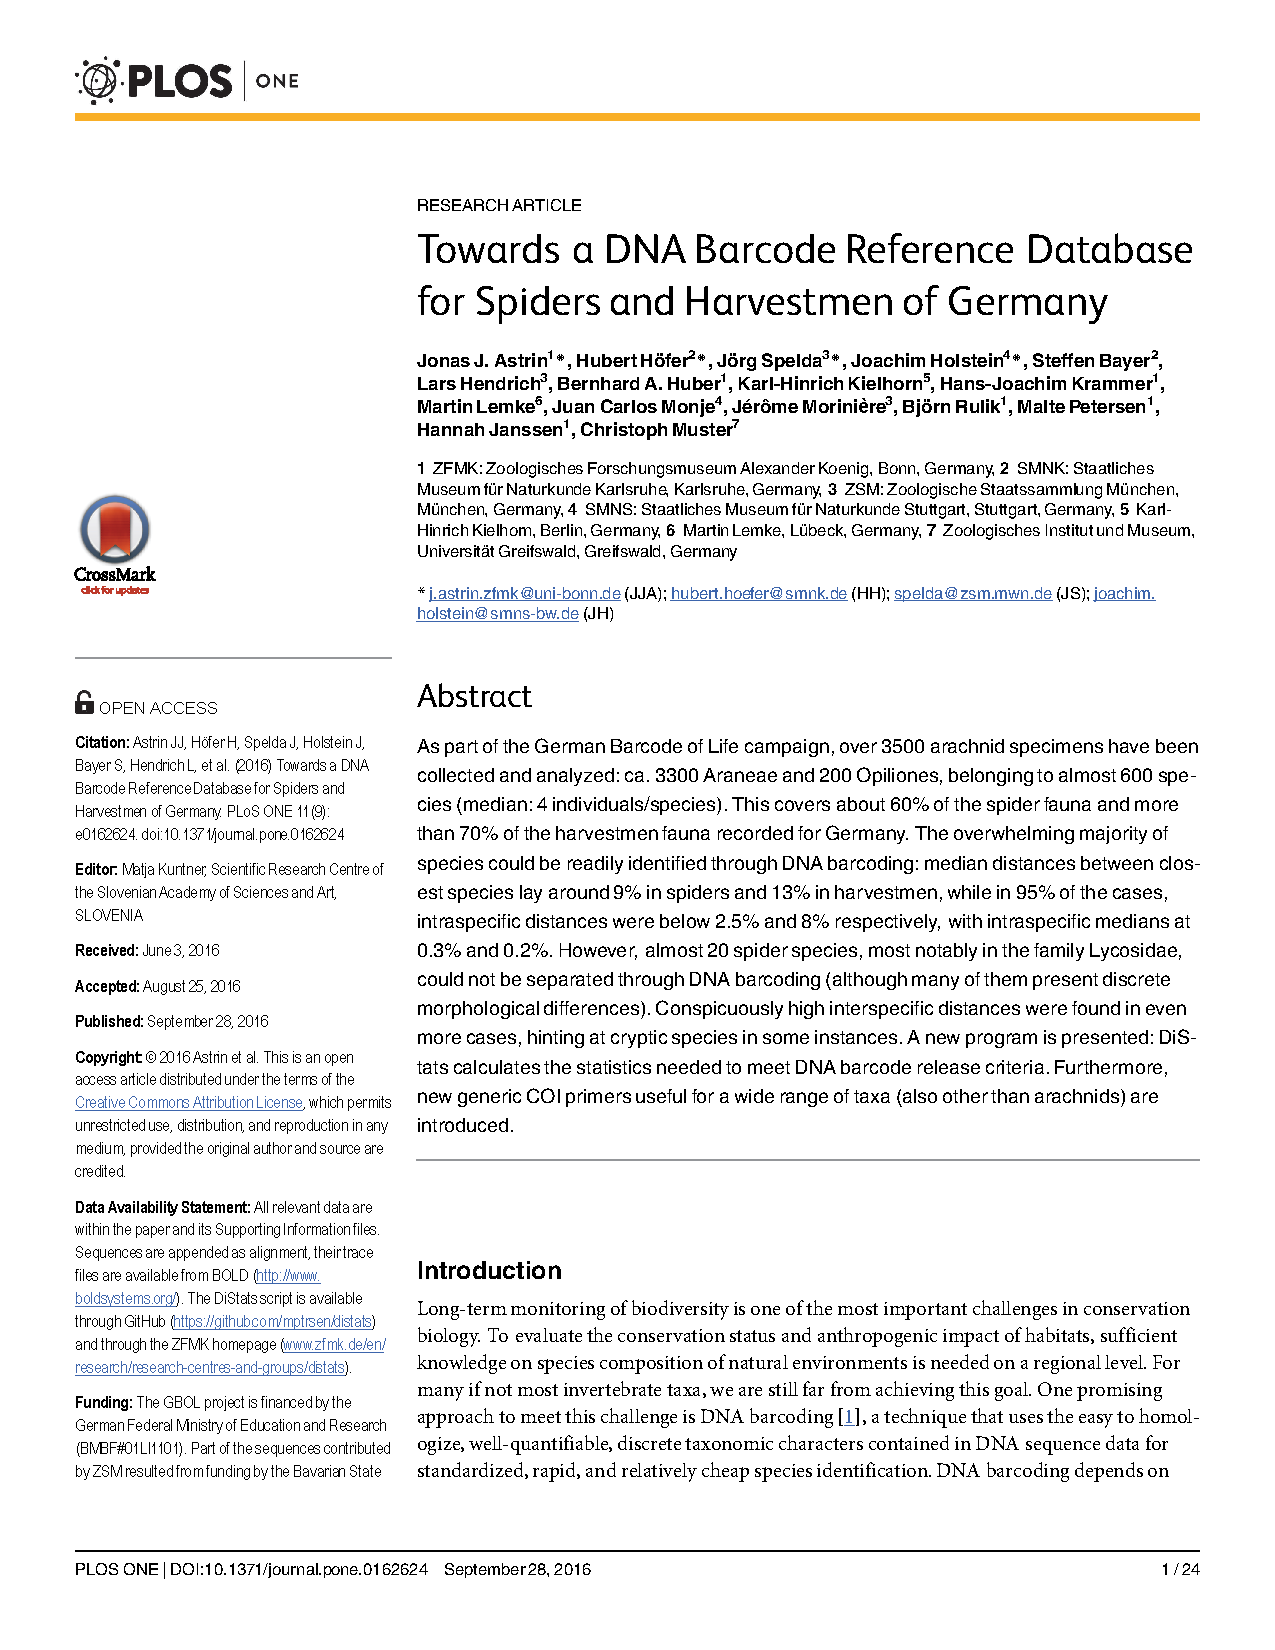
\includepdf[addtotoc={1,section,1,\citet{Astrin2016}: Towards a DNA barcode reference database for spiders and harvestmen of germany,app:Astrin2016},pages=-]{appendix/B/Astrin2016} % range without endpoints: from first to last
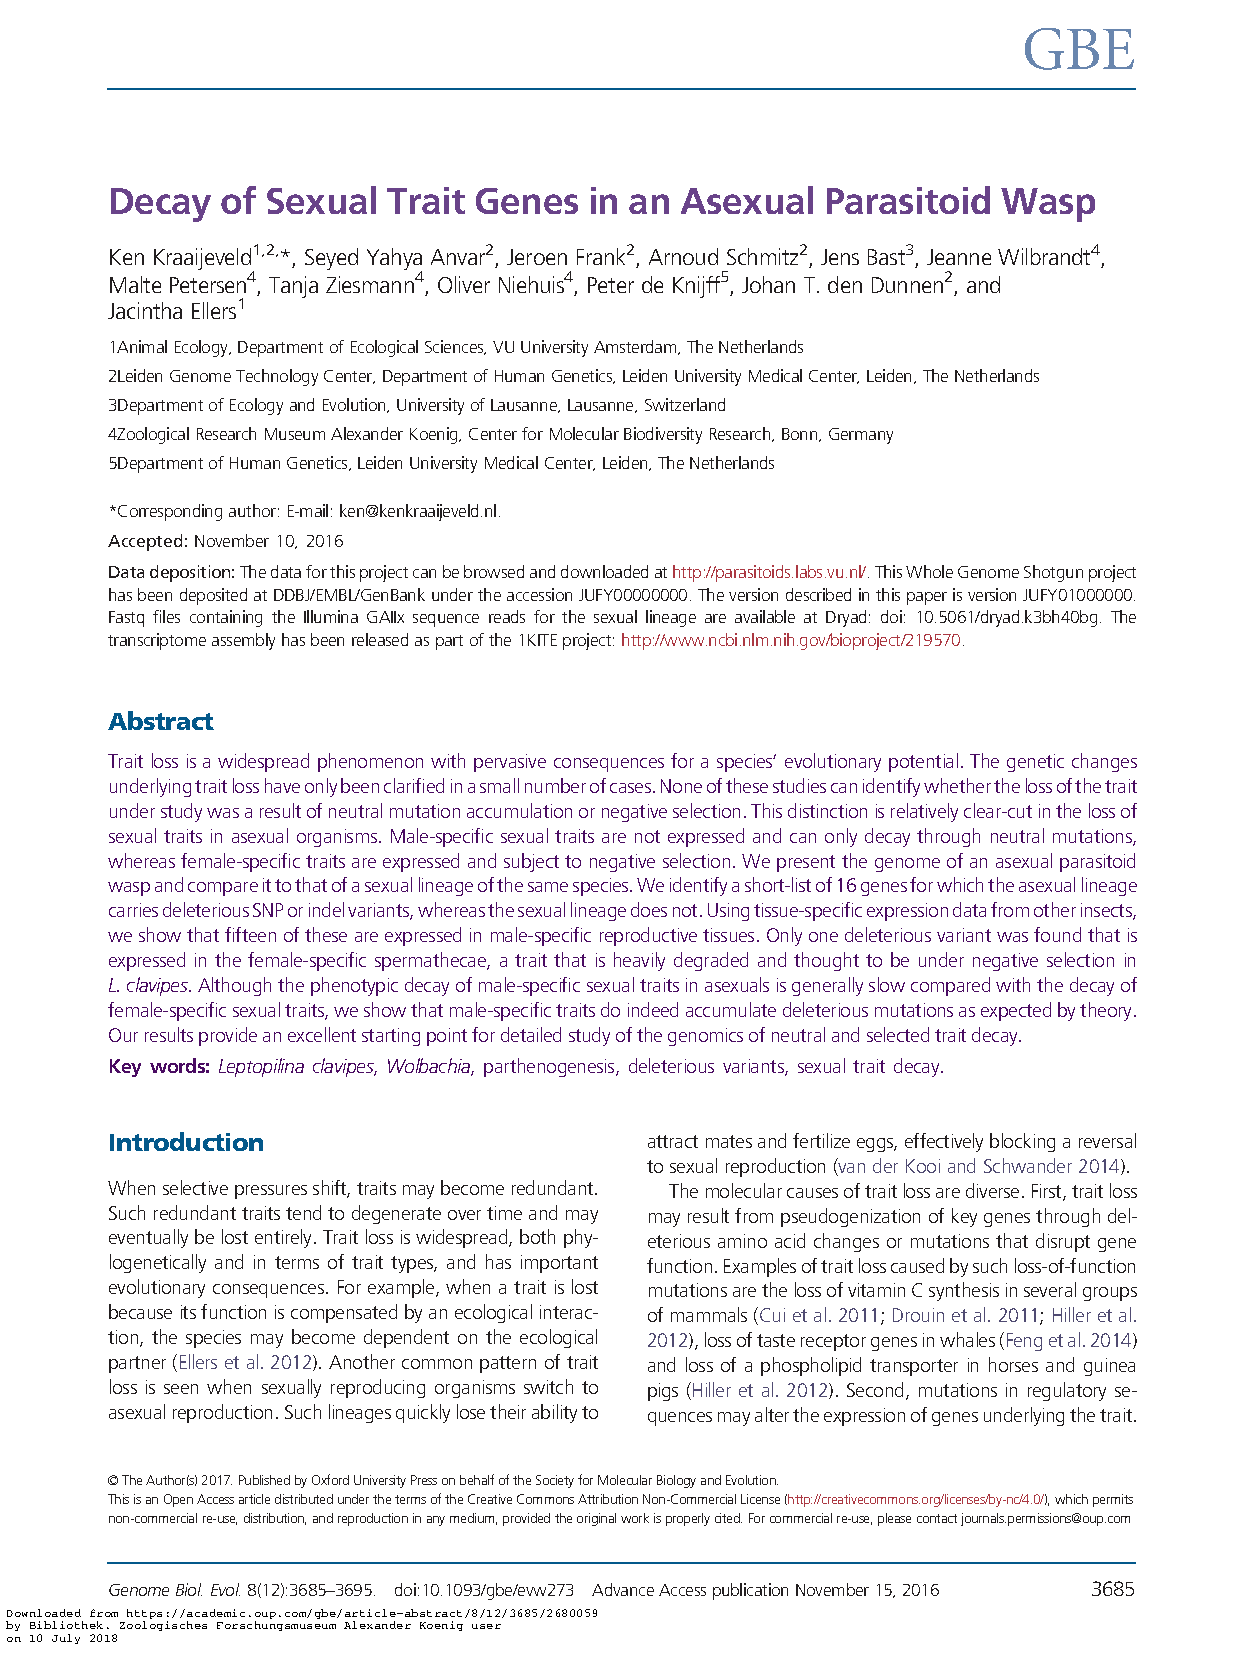
\includepdf[addtotoc={1,section,1,\citet{Kraaijeveld2016}: Decay of sexual trait genes in an asexual parasitoid wasp,app:Kraaijeveld2016},pages=-]{appendix/B/Kraaijeveld2016} % range without endpoints: from first to last
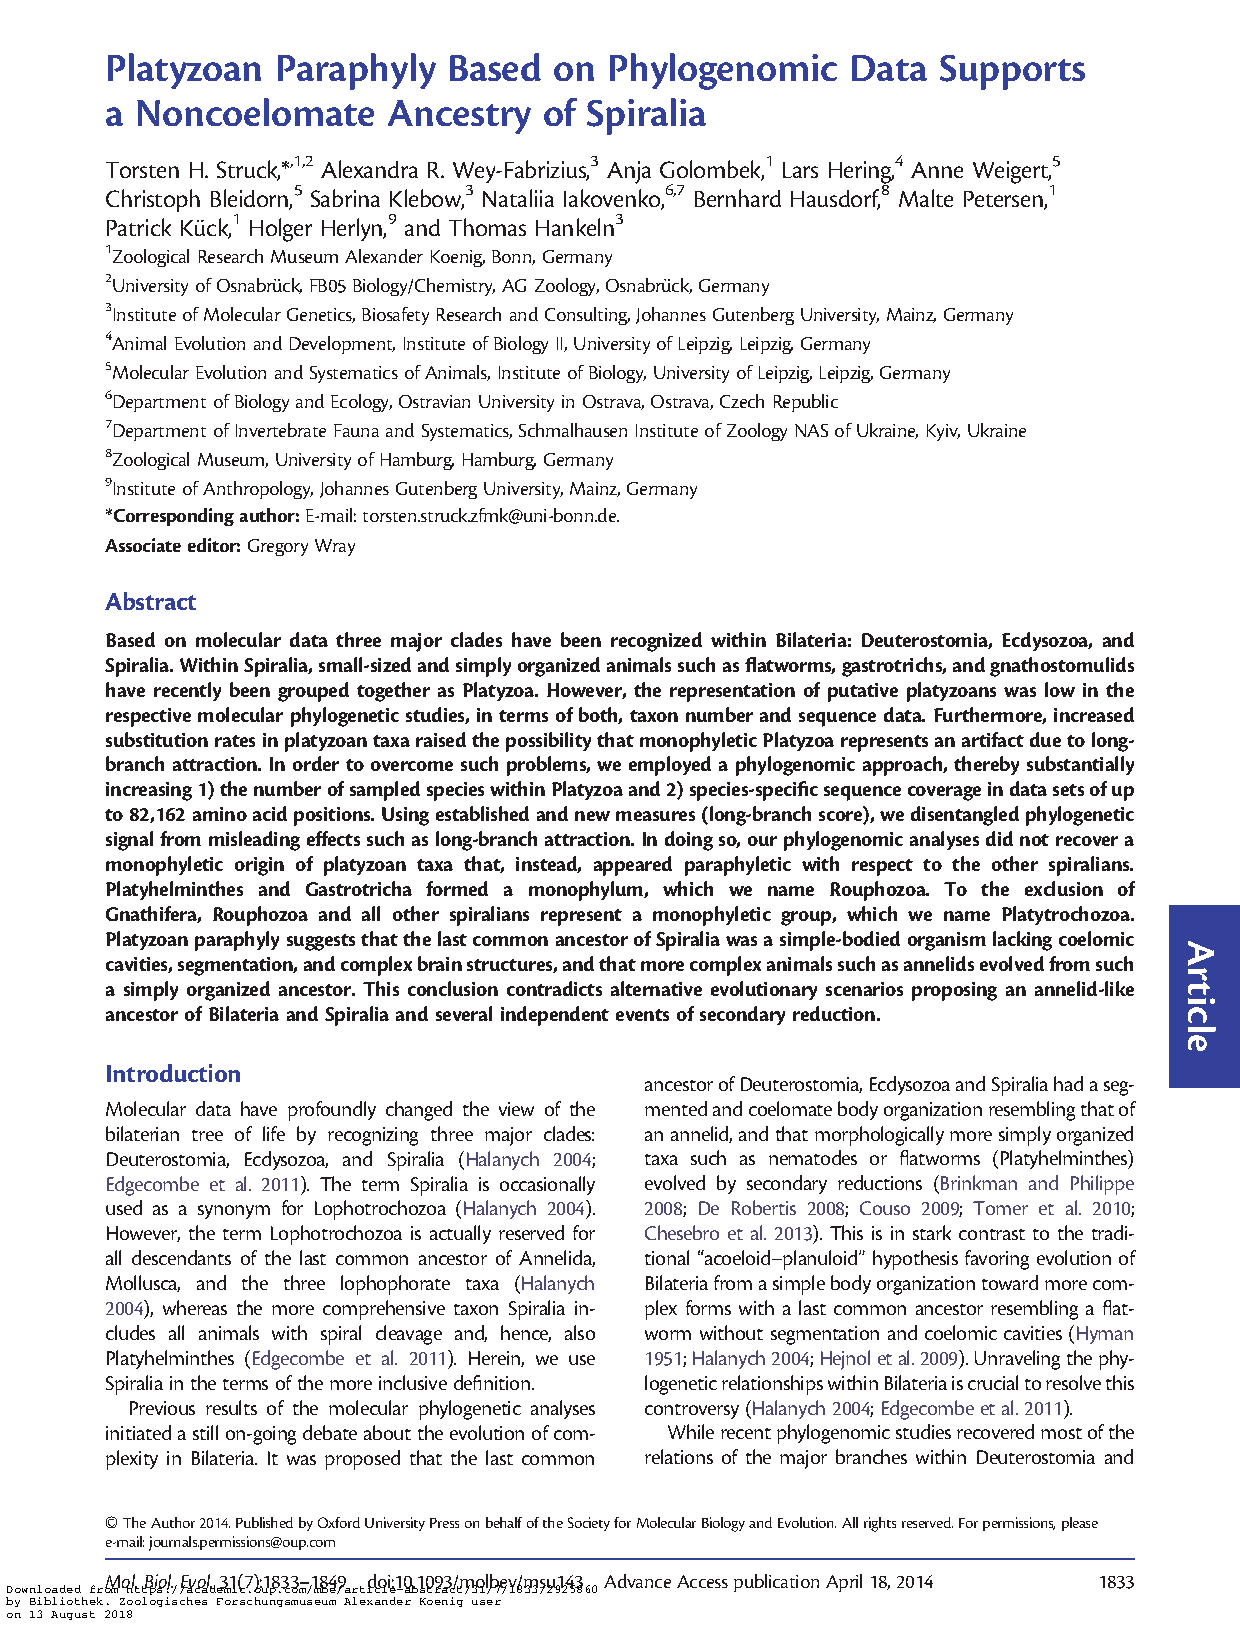
\includepdf[addtotoc={1,section,1,\citet{Struck2014}: Platyzoan paraphyly based on phylogenomic data supports a noncoelomate ancestry of Spiralia,app:Struck2014},pages=-]{appendix/B/Struck2014} % range without endpoints: from first to last
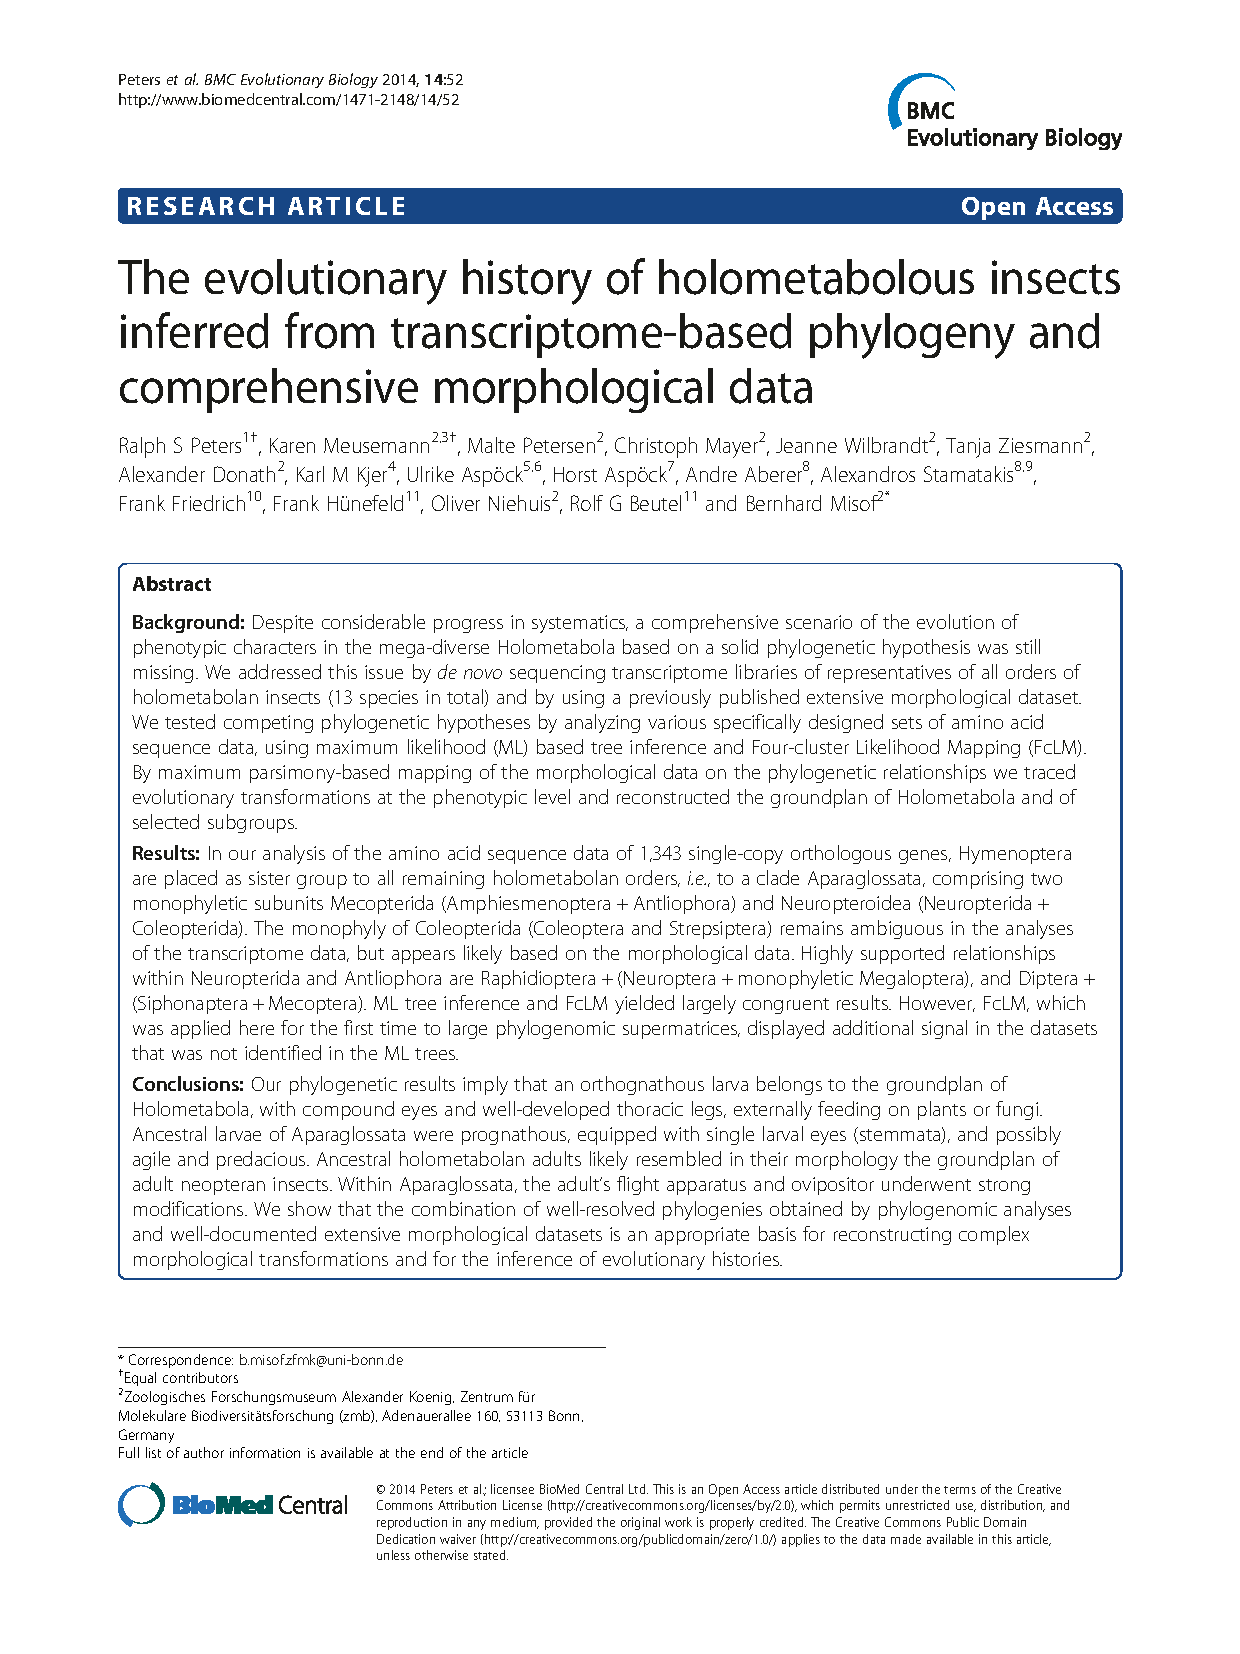
\includepdf[addtotoc={1,section,1,\citet{Peters2014}: The evolutionary history of holometabolous insects inferred from transcriptome-based phylogeny and comprehensive morphological data,app:Peters2014},pages=-]{appendix/B/Peters2014} % range without endpoints: from first to last
\label{app:Misof2014}
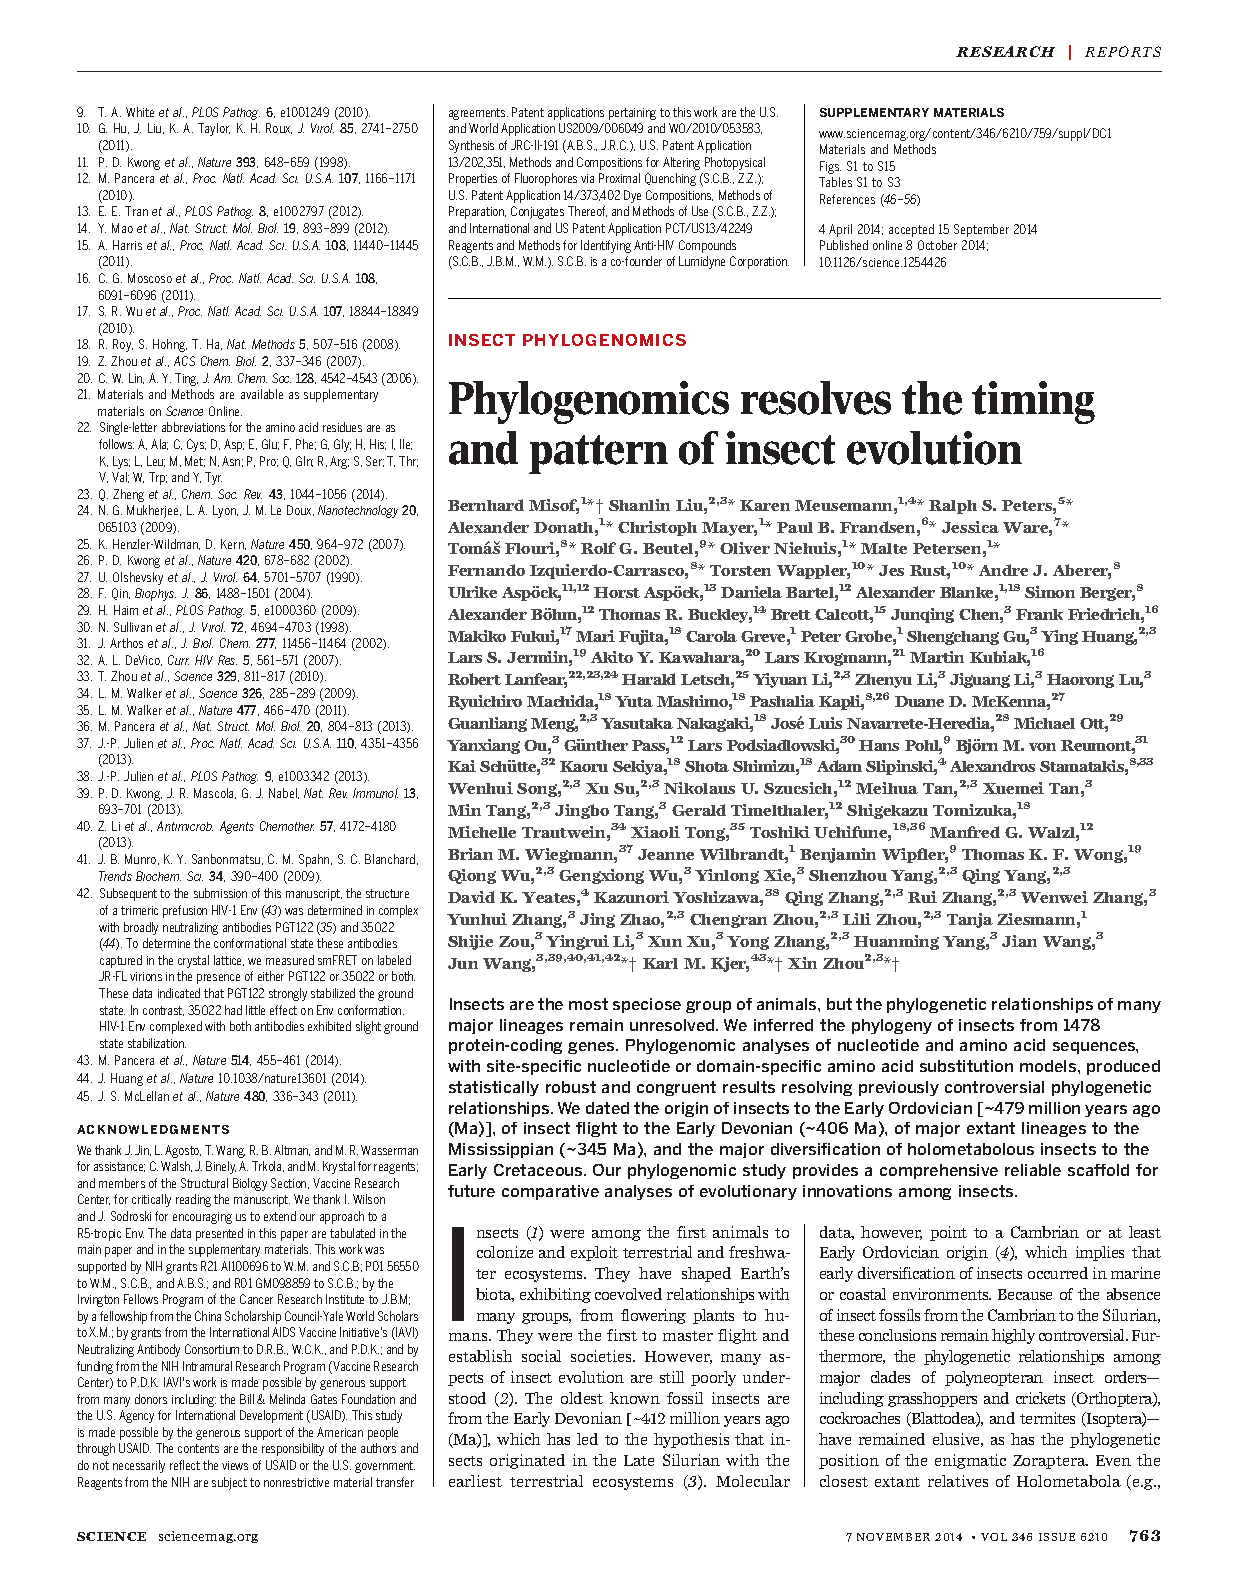
\includepdf[addtotoc={1,section,1,\citet{Misof2014}: Phylogenomics resolves the timing and pattern of insect evolution,app:Misof2014},pages=-]{appendix/B/Misof2014} % range without endpoints: from first to last
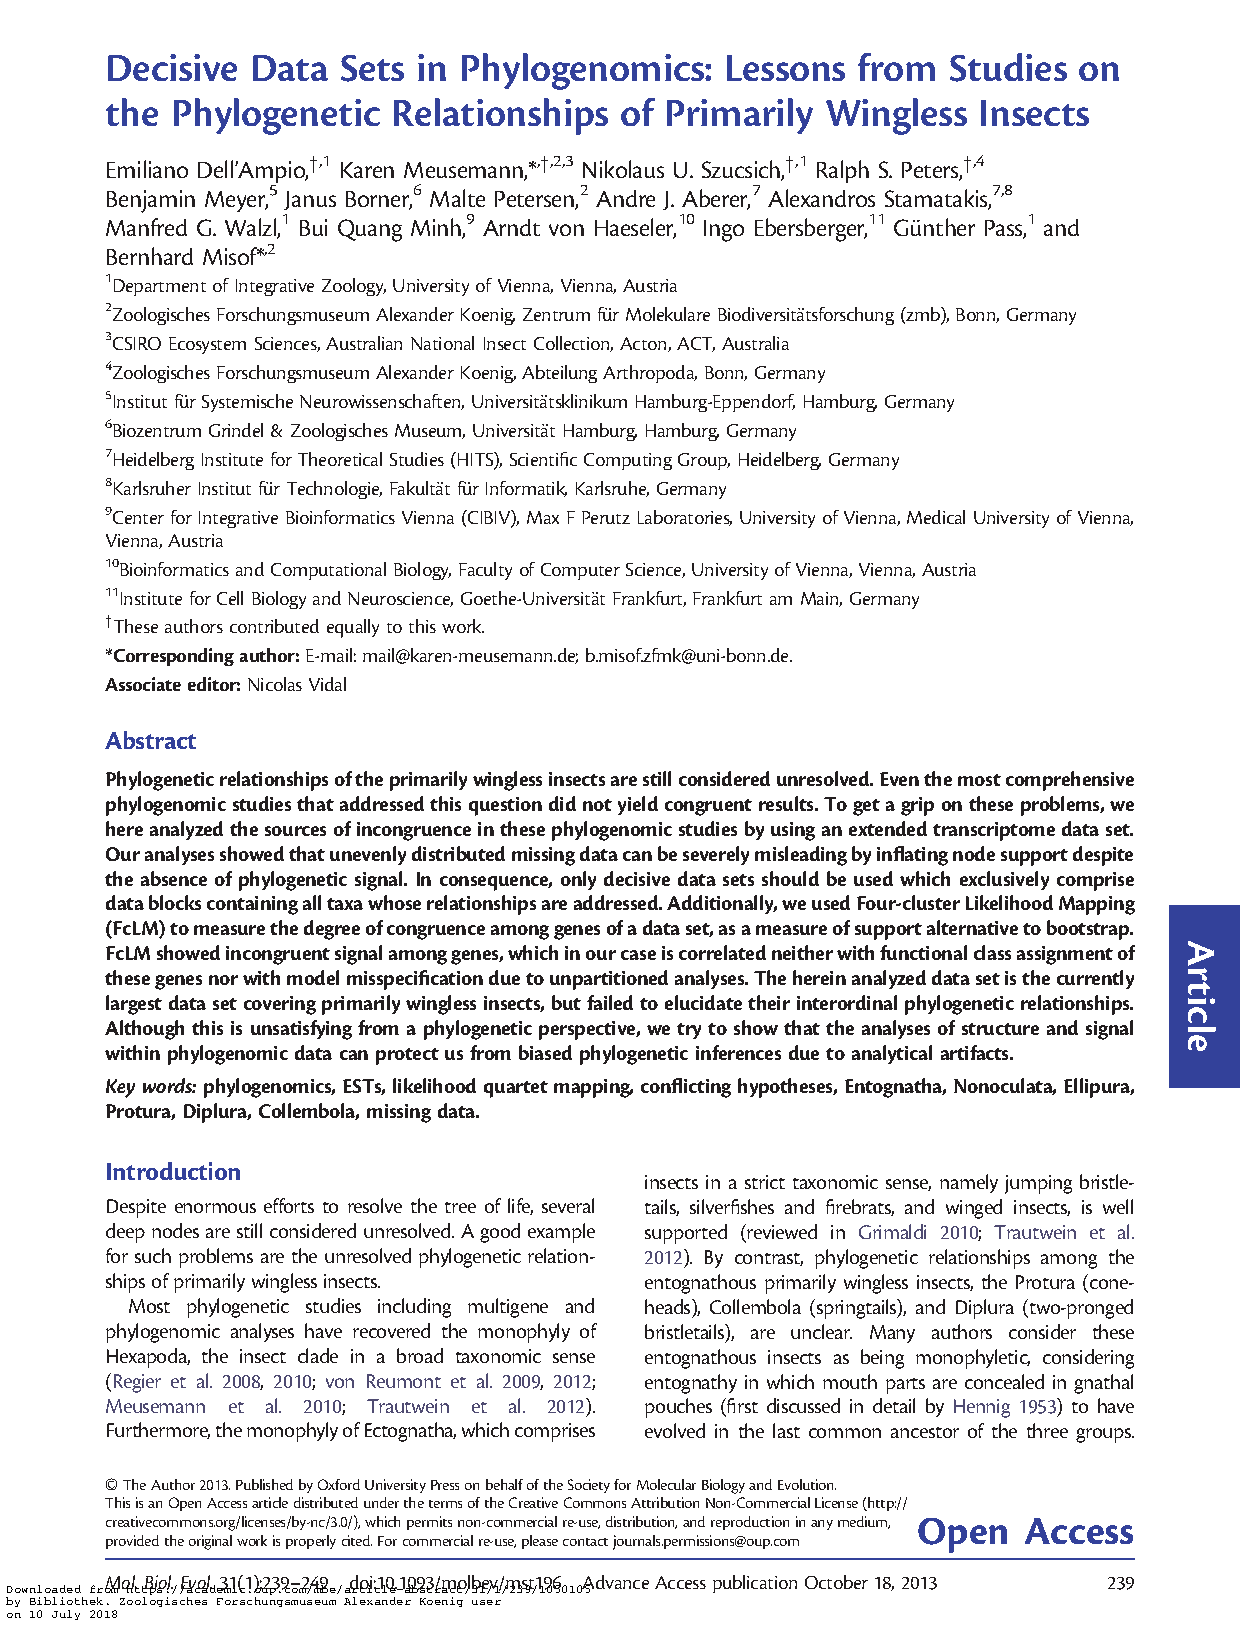
\includepdf[addtotoc={1,section,1,\citet{DellAmpio2014}: Decisive data sets in phylogenomics: lessons from studies on the phylogenetic relationships of primarily wingless insects,app:DellAmpio2014},pages=-]{appendix/B/DellAmpio2014} % range without endpoints: from first to last
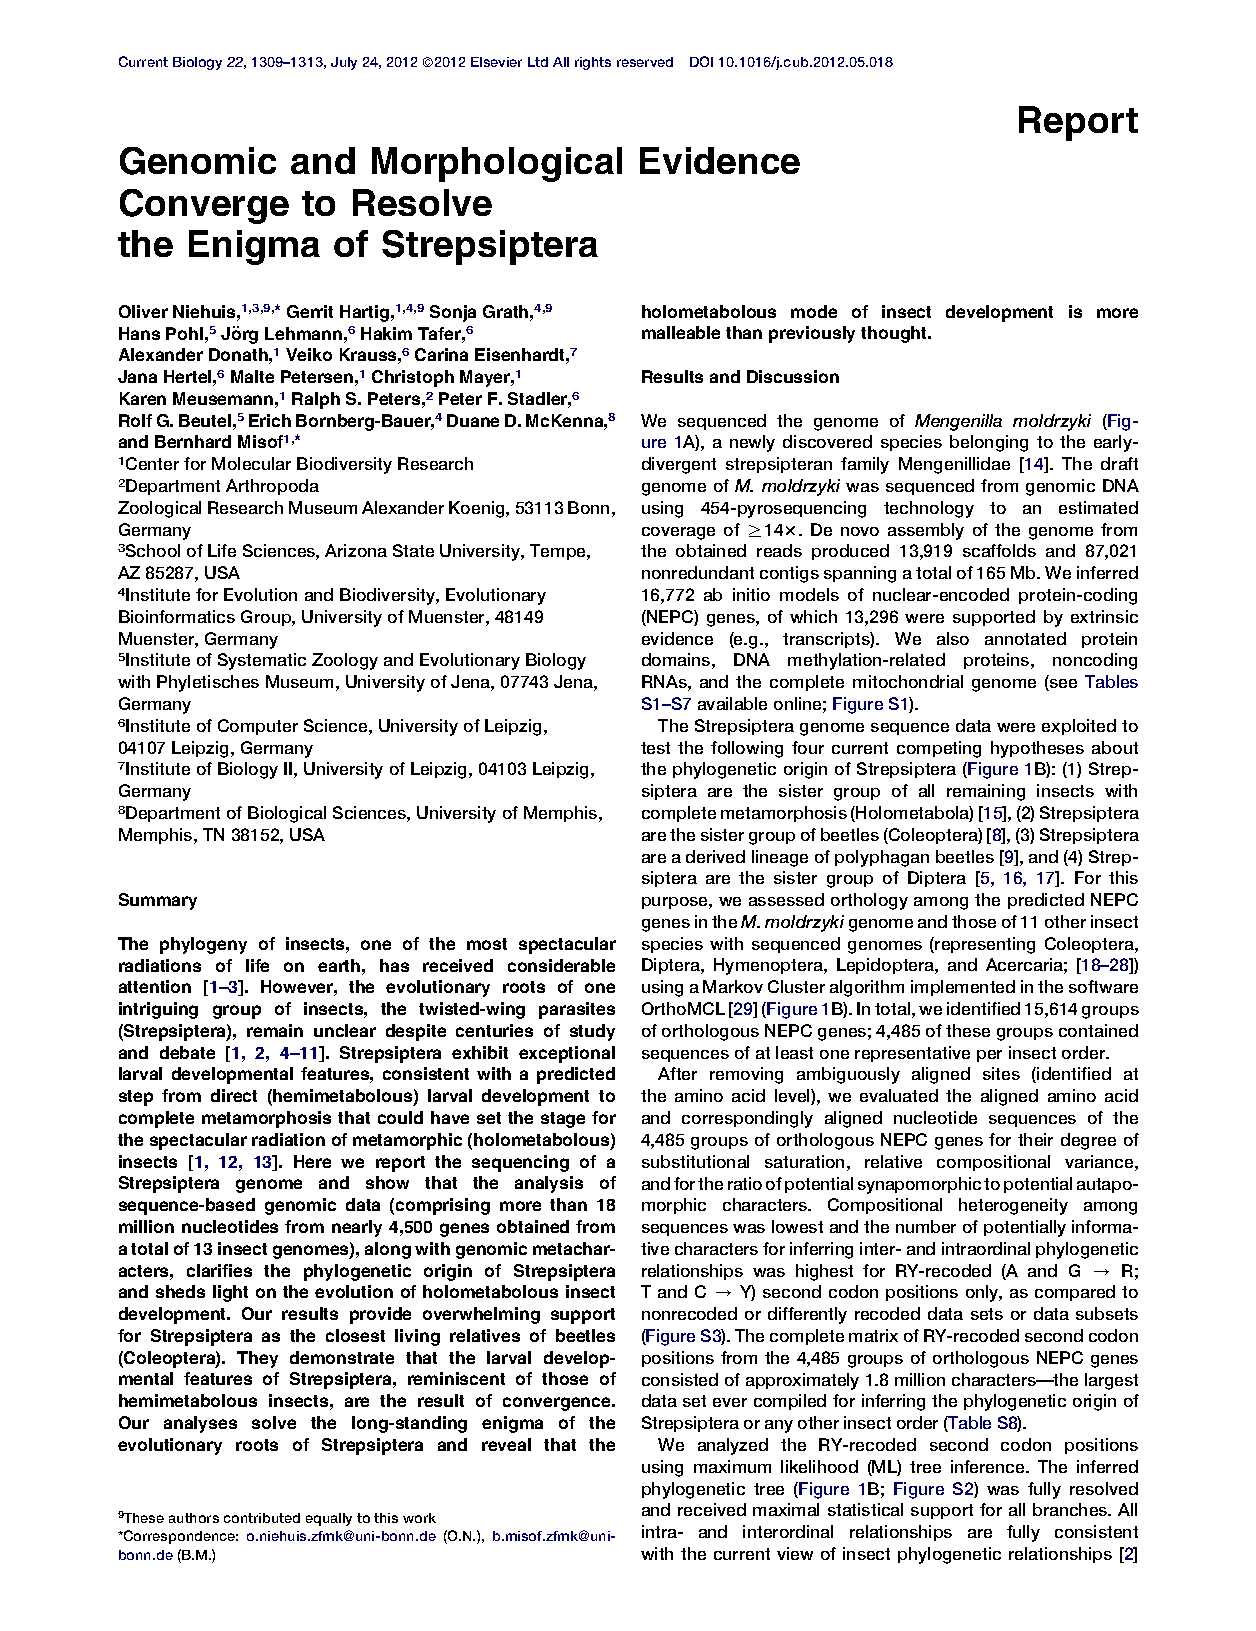
\includepdf[addtotoc={1,section,1,\citet{Niehuis2012}: Genomic and morphological evidence converge to resolve the enigma of Strepsiptera,app:Niehuis2012},pages=-]{appendix/B/Niehuis2012} % range without endpoints: from first to last
}%
